\chapter{Metodologia}
\label{ch:metodologia}

A metodologia é esquematizada na Figura~\ref{fig:metodologia} que ilustra o fluxo de trabalho. Primeiro, ocorreu a definição e compreensão do problema:
assuntos relacionados ao eletrocardiograma e ao coração. A escolha do banco envolveu selecionar um explorar um banco de dados de eletrocardiogramas 
comumente utilizado. Pré-processamento, escolha do modelo, de estratégias de validação, aplicação e avaliação dos modelos já foram atividades 
do universo de aprendizagem de máquina comumente adotadas em metodologias da área.

\begin{figure}[H]
  \centering
  \caption{Esquema da metodologia adotada.}
  \begin{tikzpicture}[node distance=1.5cm, every node/.style={draw, rounded corners, minimum width=2.8cm, minimum height=1cm, align=center}]

%passos
\node (passo0) {Definição do problema};
\node [below=of passo0] (passo1) {Escolha do banco};
\node [below=of passo1] (passo2) {Pré processamento};
\node [below=of passo2] (passo3) {Escolha dos modelos};
\node [below=of passo3] (passo4) {Escolha da estratégia de validação};
\node [below=of passo4] (passo5) {Aplicação do modelo};
\node [below=of passo5] (passo6) {Escolha do melhor modelo};

%conexões
\draw[->](passo0) -- (passo1);
\draw[->](passo1) -- (passo2);
\draw[->](passo2) -- (passo3);
\draw[->](passo3) -- (passo4);
\draw[->](passo4) -- (passo5);
\draw[->](passo5) -- (passo6);

\end{tikzpicture} % insere o tikzpicture puro
  \label{fig:metodologia}
  \legend{Fonte: Elaborado pelo autor.}
\end{figure}

Cada um desses passos introduz considerações, e as decisões tomadas influenciam nos passos seguintes. Por exemplo, a escolha do banco impacta diretamente em 
quais tipos de pré-processamento necessário, como a limpeza. Contanto, antes mesmo da escolha do banco, é necessário definir qual o problema, visto que 
que as anotações presentes podem limitar o escopo dos problemas resolvidos. 

Nas seções subsequentes, detalha-se as decisões adotadas em cada etapa da metodologia, bem como os critérios considerados para tais escolha.

\section{O banco de dados}
\label{sec:particionamento}

Dentre as opções de bancos de dados, optou-se pelo \textit{MIT-BIH Arrhythmia Database} \cite{mitbih2005}. 
O MIT-BIH é um banco aberto e muito utilizado para a classificação de arritmias, sendo o primeiro banco 
aberto de ECG da história; estando disponível desde da década de 80  \cite{moody2001}, permitindo a comparação com demais trabalhos. Além 
de ser recomendado pela AAMI \cite{chazal2004,saadatnejad2020}.


Segundo \citeonline{physionet_annotations}, o banco é composto por 58 registros de eletrocardiograma (ECG), cada um com 30 minutos de duração. 
Os 23 primeiros registros, dentro do intervalo de 100 a 124, foram selecionados aleatoriamente a partir de um conjunto de 4000 gravações de 24 horas realizadas 
em pacientes ambulatoriais do Beth Israel Deaconess Medical Center. 
Os 25 registros, dentro do intervalo de 200 a 234, restantes foram escolhidos de modo a incluir arritmias raras e com formato complexo, mas clinicamente significativas.
Cada uma das anotações foram feitas por três cardiologistas independentes. Os sinais foram coletados com duas derivações (eletrodos); uma superior e outra inferior. A superior
é majoritariamente utilizando a derivação MLII (\textit{modified limb} II) que é feita com o eletrodo no peito. 
Em alguns casos, foi utilizado as derivações V1 (ou mais raramente, V2, V3 e V4); que também são obtidas com os eletrodos no peito.

Neste trabalho, foi utilizado somente a derivação superior, pois permite uma melhor visão do complexo QRS \cite{physionet_annotations}.

Na Tabela~\ref{tab:mapeamento_classes}, é detalhado o mapeamento entre as classes originais de batimentos para as cinco definidas pela AAMI.

\begin{table}[H]
\centering
\caption{Mapeamento das anotações originais do MIT-BIH para as classes AAMI.}
\label{tab:mapeamento_classes}
\begin{tabular}{ll}
\hline
\textbf{Anotação Original} & \textbf{Classe AAMI} \\
\hline
N, e, j, L, R & N (Normal) \\
A, a, J, S & S (Supraventricular) \\
V, E & V (Ventricular) \\
F, f & F (Fusão) \\
Q, ?, / & Q (Desconhecida) \\
\hline
\end{tabular}
\legend{Fonte: Adaptado de \citeonline{chazal2004}}
\end{table}

Essas anotações são anotações de batimento, isto é, elas são feitas em cada pico R no ECG. Além delas, existem as anotações de ritmo dentre 
as quais, como o ritmo normal identificado por "(N",
e a taquicardia ventricular; identificado por "(VFL". Dentro de um contexto rítmico, podem haver batimentos normais ou arrítmicos.

Por exemplo, na Figura~\ref{fig:p100_ritmo_normal}, é mostrado o trecho de um ECG. Note a anotação de ritmo, "(N", indicando que o mesmo 
é normal. Note, também, que dentro desse contexto rítmico, existem batimentos normais, sinalizados por um ponto em cada pico R, 
uma arritmia supraventricular,
mais precisamente, o batimento atrial prematuro, classe A.

\begin{figure}[H]
  \centering
  \caption{Trecho ECG com ritmo normal do paciente 100 com arritmia classe A}
  \includegraphics[width=\linewidth]{figuras/ecg_physio_bank/p100_ritmo_normal.png}  % <-- CERTO
  \label{fig:p100_ritmo_normal}
  \legend{Fonte: Adaptado de PhysionNet}
\end{figure}

Na Figura~\ref{fig:p100_ritmo_normal_arrV} é mostrado um outro trecho do mesmo paciente, o ritmo também é normal

\begin{figure}[H]
  \centering
  \caption{Trecho ECG com ritmo normal do paciente 100 com arritmia classe V}
  \includegraphics[width=\linewidth]{figuras/ecg_physio_bank/p100_ritmo_normal_classV.png}  % <-- CERTO
  \label{fig:p100_ritmo_normal_arrV}
  \legend{Fonte: Adaptado de PhysionNet}
\end{figure}

Porém, nota-se um PVC, identificado pela anotação V. Na Figura~\ref{fig:p106_ritmo_normal_arrV}, um trecho do paciente 106 é mostrado.

\begin{figure}[H]
  \centering
  \caption{Trecho ECG com ritmo normal do paciente 106 com arritmia classe V}
  \includegraphics[width=\linewidth]{figuras/ecg_physio_bank/p106_ritmo_normal_vt_classV.png}  % <-- CERTO
  \label{fig:p106_ritmo_normal_arrV}
  \legend{Fonte: Adaptado de PhysionNet}
\end{figure}

Aqui ocorre uma taquicardia ventricular, identificado por "(VT". Nela, ocorrem três PVCs em sequência. 
Note a diferença morfológica entre eles. Após esse evento, o ritmo é normal. Nesse segundo momento, ocorre um outro PVC.

As classes de ritmo não foram utilizadas explicitamente, visto que o objetivo era classificar batimentos. Ou seja, há sequências 
com ritmo normal ou com taquicardia ventricular, mas o algoritmo não as classifica.

\section{Pré-processamento}
\label{sec:pre_process}

Antes de utilizar o sinal de ECG como entrada dos modelos, foi necessária uma etapa de pré-processamento composta por limpeza de ruídos, 
segmentação e padronização dos batimentos. Essa etapa é importante porque o ECG está sujeito a diversos ruídos que podem prejudicar o 
aprendizado das redes neurais. Como o exame registra a atividade elétrica do coração, correntes elétricas externas ou internas ao organismo 
podem modificar o sinal. Entre os ruídos mais comuns estão o ruído muscular (proveniente da contração de outros músculos), o \textit{baseline wander} 
(variação lenta associada à respiração) e a interferência de 60 Hz da rede elétrica, como discutido na seção \ref{sec:trabalhos_correlatos}.

Apesar disso, alguns trabalhos utilizam o sinal praticamente cru, delegando ao próprio modelo o papel de identificar o que é ou não relevante. 
Essa abordagem simplifica o pré-processamento, mas aumenta a complexidade do problema de aprendizado e pode demandar bases maiores ou arquiteturas 
mais robustas.

Outro desafio importante é a segmentação do ECG em batimentos individuais. Conforme observado nos trabalhos correlatos, existem duas abordagens 
principais: o uso de janelas de tempo fixas ou janelas adaptadas ao tamanho do batimento. Janelas fixas são simples, mas podem cortar partes 
importantes do complexo QRS ou incluir trechos de batimentos vizinhos. Em ambas as estratégias, o pico R é normalmente utilizado como referência. 
Uma vantagem do MIT-BIH é que esses picos já estão anotados; quando não estão, podem ser identificados por algoritmos como o de 
\citeonline{pantompkins1985}.

Neste trabalho, optou-se por trabalhar com o sinal o mais próximo possível do original, preservando suas características fisiológicas e 
facilitando análises posteriores. Por isso, adotou-se a segmentação flexível. Inicialmente, o sinal foi limpo com um filtro passa-alta de 
0,5 Hz (ordem 5), seguido de filtragem da linha de energia a 60 Hz. Em seguida, foi executada a segmentação. Ambas as etapas utilizaram a 
biblioteca NeuroKit2 \cite{Makowski2021neurokit}.

Por fim, foi necessário uniformizar o tamanho dos batimentos antes de alimentá-los nos modelos. A média das amostras por batimento foi de 
aproximadamente 284; portanto, adotou-se uma reamostragem para 288 amostras, correspondendo a 800 ms de duração. Essa etapa foi realizada com a 
função \textit{resample} da biblioteca SciPy \cite{2020SciPy-NMeth}.

Na figura abaixo é ilustrado um batimento segmentado e limpo e o seu trecho correspondente crú.

\begin{figure}[h!]
    \centering
    \caption{Comparação entre o ECG original, segmentado e reamostrado}
    \begin{minipage}{0.5\textwidth}
        \centering
        \includegraphics[width=\linewidth]{figuras/ecg_physio_bank/p101_batimentoSegmentadoVsOrignal.png}
        \subcaption{ECG crú e segmentado}
        \label{fig:image1}
    \end{minipage}%
    \begin{minipage}{0.5\textwidth}
        \centering
        \includegraphics[width=\linewidth]{figuras/ecg_physio_bank/p101_segmentadovsAmostrado.png} 
        \subcaption{ECG segmentado e reamostrado}
        \label{fig:image2}
    \end{minipage}
    \label{fig:twoimages}
    \legend{Fonte: Elaborado pelo autor.}
\end{figure}

\subsection{\textit{Features}}

Após o pré-processamento, é necessário avaliar quais \textit{features} devem ser utilizadas. Em problemas de ECG, essas \textit{features} 
precisam ser relevantes para o domínio clínico. Por outro lado, redes neurais apresentam a vantagem de aprender representações diretamente dos 
dados brutos, o que reduz a necessidade de engenharia manual de atributos. Ainda assim, algumas \textit{features} simples podem complementar o aprendizado, 
fornecendo informação explícita que ajude o modelo a distinguir padrões.

Neste trabalho, optou-se por utilizar apenas o intervalo RR como feature adicional, permitindo que a própria rede aprenda as demais 
características relevantes a partir do sinal segmentado. O intervalo RR é uma informação particularmente útil porque descreve o tempo entre 
batimentos consecutivos. Essa informação ajuda na identificação de arritmias cuja principal manifestação é temporal, como no caso dos batimentos 
ventriculares prematuros (PVCs), em que ocorre um encurtamento característico desse intervalo.

Assim, para um batimento \textit{i}, seu intervalo RR é calculado da seguinte forma.

\begin{equation}
\text{pré RR intervalo} = |R_{i-1} - R_{i}|
\end{equation}

\begin{equation}
\text{pós RR intervalo} = |R_{i} - R_{i+1}|
\end{equation}

Note que é necessário saber sobre o próximo batimento, isto é o futuro. Em um contexto de classificação em tempo real, 
por exemplo, isso poderia ser um vazamento, o que não é o caso deste projeto.

\section{Arquiteturas}
\label{sec:modelos}

Após o pré-processamento e a definição das \textit{features}, foi necessário escolher as arquiteturas de rede neural que serão avaliadas. 
Como discutido por \citeonline{geron2022hands}, a busca por hiperparâmetros ideais e por configurações de modelo costuma ser um processo 
altamente experimental, podendo incluir técnicas automáticas — como \textit{ grid search} ou \textit{random search} —, mas que, 
no contexto de redes neurais profundas, frequentemente se torna inviável devido ao custo computacional.

Uma alternativa prática consiste em partir de arquiteturas já propostas na literatura e adaptá-las ao problema estudado. 
Seguindo essa estratégia, para o modelo recorrente puro foi adotada como referência a arquitetura apresentada em \citeonline{narotamo2024}. 
No trabalho original, os autores utilizam três camadas de GRUs, cada uma com 256 unidades ocultas, explorando a capacidade das redes recorrentes 
de modelar dependências temporais no sinal.

Neste projeto, a arquitetura base foi mantida, mas além de receber o sinal do eletrocardiograma, o modelo recebeu também os intervalos RR.

A Figura~\ref{fig:gru_pura} apresenta um esquema da arquitetura utilizada.

\begin{figure}[H]
  \centering
  \caption{Arquitetura GRU pura.}
  \begin{tikzpicture}[node distance=1.5cm, every node/.style={draw, rounded corners, minimum width=2.8cm, minimum height=1cm, align=center}]

\node (input){Entrada ECG e intervalo RR};
\node [below=of input](gru_1){GRU};
\node [below=of gru_1](gru_2){GRU};
\node [below=of gru_2](gru_3){GRU};
\node [below=of gru_3](saida){Classificação final};

%conexões:

\draw[->](input) -- (gru_1);
\draw[->](gru_1) -- (gru_2);
\draw[->](gru_2) -- (gru_3);
\draw[->](gru_3) -- (saida);
\end{tikzpicture}
 % insere o tikzpicture puro
  \label{fig:gru_pura}
  \legend{Fonte: Elaborado pelo autor.}
\end{figure}

A segunda arquitetura avaliada é um modelo híbrido composto por camadas convolucionais seguidas de uma camada recorrente do tipo GRU. Nessa abordagem, o bloco convolucional é aplicado individualmente a cada batimento da sequência, gerando para cada um deles um mapa de \textit{features} que, em seguida, compõe a nova sequência processada pelo bloco recorrente.

O bloco convolucional é formado por duas camadas de CNN: a primeira com 32 filtros e \textit{kernel} de tamanho sete, e a segunda com 64 filtros e \textit{kernel} de tamanho cinco, ambas utilizando \textit{padding} adequado para preservar o comprimento da entrada. A escolha do tamanho do filtro, ou \textit{kernel}, 
envolve a escolha entre padrões globais, com um \textit{kernel} maior, ou padrões mais locais, com um \textit{kernel} menor. Arquiteturas profundas costumam usar kernels pequenos. Como esta tem apenas duas camadas, foi utilizado um de tamanho sete, e outro de tamanho cinco.

Cada camada convolucional é seguida por \textit{batch normalization} — para estabilizar o treinamento — e por \textit{global max pooling}, que reduz a dimensionalidade do mapa de \textit{features} e contribui para mitigar sobreajuste ao reter apenas as ativações mais relevantes.

A etapa recorrente é composta por uma camada GRU com 256 unidades, responsável por modelar a dependência temporal entre os batimentos por meio das representações produzidas pelo bloco convolucional.

Essa arquitetura representa uma versão simplificada do modelo proposto por \citeonline{narotamo2024}. 

\begin{figure}[H]
  \centering
  \caption{Arquitetura híbrida CNN e GRU.}
  \begin{tikzpicture}[node distance=1.5cm, every node/.style={draw, rounded corners, minimum width=2.8cm, minimum height=1cm, align=center}]

% Entradas
\node (morf) {Entrada Morfológica (ECG)};
\node[right=of morf] (ritmo) {Entrada features};

%blocos de redes neurais:
\node[below=1.5cm of morf] (cnn) {Bloco CNN \\ (extração morfológica)};

% Combinação
\node[below=1.5cm of cnn, xshift=2.5cm] (fusion) {Combinação das Saídas};

% Bloco RNN
\node[below=of fusion] (rnn) {Bloco GRU \\ (padrões temporais)};

%saída
\node[below=of rnn] (saida) {Classificação Final};

%conexões
\draw[->](morf) -- (cnn);
\draw[->](cnn) -- ++ (fusion);
\draw[->](ritmo) -- ++ (fusion);
\draw[->](fusion) -- (rnn);
\draw[->](rnn) -- (saida);

\end{tikzpicture}

 % insere o tikzpicture puro
  \label{fig:cnn_gru}
  \legend{Fonte: Elaborado pelo autor.}
\end{figure}

Enquanto que a rede da Figura~\ref{fig:gru_pura} recebeu o ECG concatenado com as \textit{features}, a rede híbrida as recebeu separadas, sendo conectadas após o processamento
das CNNs já que o objetivo era que esta extraísse \textit{features} morfológicas.

\subsection{Tamanho da sequência}

Para otimizar o processo de treinamento, foram empregados os mecanismos de \textit{early stopping} e \textit{reduce on plateau}, responsáveis por limitar o número de épocas e ajustar dinamicamente a taxa de aprendizagem, respectivamente. Ambos monitoraram o \textit{f1-score}, de forma que a rede buscasse um equilíbrio entre precisão e \textit{recall}. Assim, mesmo após o treinamento, era possível ajustar manualmente esse compromisso com auxílio da curva PR.

Em ambos os modelos, utilizou-se uma sequência composta por 16 batimentos, sendo a classificação realizada apenas no último elemento da sequência. Dessa forma, o problema caracteriza-se como uma tarefa de sequência para vetor, conforme discutido na Seção~\ref{sec:fundamentos_rnn}.

A escolha do tamanho da sequência foi feita empiricamente. Inicialmente, avaliou-se uma arquitetura simples — uma única camada de LSTM com 100 unidades — utilizando uma validação cruzada one hold out. Embora validações com mais \textit{folds} reduzam o viés na estimativa de generalização, conforme \citeonline{james2023}, o custo computacional cresce proporcionalmente, o que motivou a escolha desse arranjo mais enxuto para experimentação inicial.

Foram testadas sequências de 10, 16 e 20 batimentos. Houve melhora de desempenho ao passar de 10 para 16 batimentos, porém o aumento para 20 resultou em um consumo de memória excessivamente elevado, sem ganho proporcional. Por esse motivo, definiu-se o tamanho final da sequência como 16 batimentos.

As redes foram treinadas por até 50 épocas.

\section{Estratégia de avaliação}

Em seguida, é preciso escolher uma estratégia de avaliação. Conforme apresentado na seção \ref{sec:trabalhos_correlatos},
existem duas estratégias principais: a interpaciente e a intra-paciente. Na primeira, o modelo é exposto a um cenário mais realista,
ele é treinado em um conjunto de pacientes e avaliado em outro. O desafio reside justamente na variabilidade dos tipos arrítmicos. 
Assim, \citeonline{chazal2004}
propôs dois conjuntos de dados para o MIT-BIH; o Ds1 que é formado pelos pacientes: 101, 106, 108, 109, 112, 114, 115, 116, 118, 119, 122, 124, 201, 203, 205, 207, 208, 209, 215, 220, 223 e 230
e o Ds2, formado por: 100, 103, 105, 111, 113, 117, 121, 123, 200, 202, 210, 212, 213, 214, 219, 221, 222, 228, 231, 232, 233 e 234.

Note que o conjunto Ds1 inclui 12 registros que são resultados da seleção aleatória e 10 dos registros com as morfologias complexas. Já no Ds2 possui 
oito dessa primeira seleção e 14 da segunda; sendo mais desafiador e feito para testar a capacidade de generalização do modelo.

Na Tabela~\ref{tab:particionamento}, é mostrado a distribuição das classes usadas pelos modelos; a arritmia ventricular e a normal.

\begin{table}[htb]
\centering
\caption{Distribuição das classes (por batimento) nos conjuntos Ds1 e Ds2}
\label{tab:particionamento}
\begin{tabular}{|l|c|c|}
\hline
Conjunto & N & VEB \\ \hline
DS1 & 45\,866 & 3\,788 \\ \hline
DS2 & 44\,259 & 3\,221 \\ \hline
Total & 90\,125 & 7\,009 \\ \hline
\end{tabular}
\legend{Fonte: o autor.}
\end{table}


\iffalse
\begin{table}[htb]
\centering
\caption{Distribuição das classes nos conjuntos Ds1 e Ds2}
\label{tab:particionamentoOld}
\begin{tabular}{|l|c|c|c|c|c|c|}
\hline
Conjunto & N & SVEB & VEB & F & Q & Total \\ \hline
DS1 & 45 866 & 944 & 3 788 & 415 & 8 & 51 021 \\ \hline
DS2 & 44 259 & 1 837 & 3 221 & 388 & 7 & 49 712 \\ \hline
Total & 90 125 & 2 781 & 7 009 & 803 & 15 & 100 733 \\ \hline
\end{tabular}
\legend{Fonte: o autor.}
\end{table}
\fi

Como pode ser observado, as classes são desbalanceadas dentro do mesmo conjunto, porém, balanceada entre eles.

A avaliação foi feita utilizando uma avaliação cruzada no conjunto Ds1 inicialmente com duas partições (dois \textit{folds}) e, posteriormente, com cinco partições (cinco \textit{folds}) nos modelos finais, utilizando o particionados
inter-paciente. Esta estratégia permite avaliar o modelo com ECGs de pacientes para o qual ele não foi treinado; sendo mais próximo de um contexto clínico 
e expõe o modelo a mais variação. Além disso, conforme a AAMI, batimentos com marcapasso foram excluídos por serem não representativos \cite{saadatnejad2020}.

Na Tabela~\ref{tab:folds}, abaixo, é mostrado os pacientes em cada \textit{fold}.

\begin{table}[htbp]
    \centering
    \caption{Distribuição dos IDs dos Pacientes por Fold para Conjuntos de Treinamento e Validação}
    \label{tab:folds}
    \small % Reduz o tamanho da fonte da tabela para melhor encaixe
    \begin{tabular}{|>{\centering\arraybackslash}p{1.5cm}|>{\raggedright\arraybackslash}p{7.5cm}|>{\raggedright\arraybackslash}p{5.5cm}|}
        \toprule
        \textbf{Fold} & \textbf{Conjunto de Treinamento} & \textbf{Conjunto de Validação} \\
        \midrule
        1 & 101, 106, 108, 109, 112, 114, 116, 119, 122, 124, 203, 205, 207, 208, 209, 215, 220, 223 & 115, 118, 201, 230 \\
        \midrule
        2 & 101, 108, 109, 112, 114, 115, 116, 118, 119, 201, 203, 205, 207, 208, 209, 215, 220, 223, 230 & 106, 122, 124 \\
        \midrule
        3 & 101, 106, 108, 109, 112, 114, 115, 116, 118, 122, 124, 201, 207, 208, 215, 220, 223, 230 & 119, 203, 205, 209 \\
        \midrule
        4 & 106, 112, 114, 115, 118, 119, 122, 124, 201, 203, 205, 207, 208, 209, 215, 230 & 101, 108, 109, 116, 220, 223 \\
        \midrule
        5 & 101, 106, 108, 109, 115, 116, 118, 119, 122, 124, 201, 203, 205, 209, 220, 223, 230 & 112, 114, 207, 208, 215 \\
        \bottomrule
    \end{tabular}
    \legend{Fonte: o autor.}
\end{table}

\subsection{Métricas}
\label{sec:metricas}

As métricas utilizadas para avaliar o desempenho dos modelos foram selecionadas em duas categorias: métricas de desempenho 
(sensibilidade, precisão, acurácia, \textit{F1-score}, AUC, AP), que quantificam os tipos de acertos e erros, e métricas de confiabilidade 
(curva de calibração), que avaliam a coerência das probabilidades previstas. 
Para iniciar, será apresentada a matriz de confusão, que serve como fundamento para as métricas de desempenho ao tipificar os acertos e erros 
do modelo em termos de verdadeiros e falsos.

\subsubsection{Matriz de confusão e métricas derivadas}

Na Tabela~\ref{tab:matriz_confusao} é ilustrada um exemplo de matriz de confusão para um classificador binário.

\begin{table}[H]
\centering
\caption{Exemplo de matriz de confusão binária}
\label{tab:matriz_confusao}
\begin{tabular}{|c|c|c|}
\hline
\multirow{2}{*}{\textbf{Classe Verdadeira}} & \multicolumn{2}{c|}{\textbf{Classe Predita}} \\ \cline{2-3} 
 & Positiva & Negativa \\ \hline
Positiva & TP & FN \\ \hline
Negativa & FP & TN \\ \hline
\end{tabular}
\legend{Fonte: Elaborado pelo autor.}
\end{table}

Segundo \citeonline{Mueller2016}, cada quadrante da matriz representa um tipo de acerto ou erro, a saber:

\begin{enumerate}
\item {TP} (\textit{true positive} - verdadeiro positivo), quantos casos positivos foram corretamente classificados;
\item {FN} (\textit{false negative} - falso negativo), quantos casos negativos foram incorretamente classificados;
\item {FP} (\textit{false positive} - falso positivo), quantos casos positivos foram incorretamente classificados;
\item {TN} (\textit{true negative} - verdadeiro negativo), quantos casos negativos foram corretamente classificados.
\end{enumerate}

E com base nesses tipos, são definidas as seguintes métricas de desempenho(\cite{Mueller2016}):

\noindent\textbf{Acurácia:} Corresponde ao acerto global do modelo:
\begin{equation}
\text{Acurácia} = \frac{TP + TN}{TP + TN + FP + FN}
\end{equation}

\noindent\textbf{Sensibilidade (\textit{recall}):} Representa a capacidade do modelo em identificar corretamente a classe positiva, sendo $\text{TPR}$ (Taxa de Verdadeiros Positivos) seu sinônimo.
\begin{equation}
\text{Sensibilidade} = \frac{TP}{TP + FN}
\end{equation}

\noindent\textbf{Precisão:} Indica a proporção de amostras classificadas como positivas que realmente pertencem à classe positiva:
\begin{equation}
\text{Precisão} = \frac{TP}{TP + FP}
\end{equation}

\noindent\textbf{\textit{F1-score}:} É a média harmônica entre precisão e sensibilidade, buscando um equilíbrio entre as duas:
\begin{equation}
\text{\textit{F1-score}} = \frac{2 \cdot \text{Precisão} \cdot \text{Sensibilidade}}{\text{Precisão} + \text{Sensibilidade}}
\end{equation}

\subsubsection{Curva de Precisão e Recall}

Segundo \citeonline{geron2022hands}, a precisão e o \textit{recall} são um \textit{trade-off}; conforme aumenta-se o \textit{recall},
a tendência é que o modelo comete mais erros de falsos positivos, diminuindo a precisão. Da mesma forma, conforme aumenta-se a precisão, 
o modelo tende a cometer mais erros de falsos negativos, diminuindo a sensibilidade.

Em \citeonline{Mueller2016}, chama-se a atenção para qual tipo de erro é menos danoso, pois nenhum modelo é livre de erros.
Em contextos médicos, prioriza-se o \textit{recall}, pois falsos negativos são mais prejudiciais que falsos positivos. 
Segundo os autores, uma forma de visualizar esse \textit{trade-off} é pela curva precisão-\textit{recall}, ilustrada abaixo, que 
mostra o desempenho do modelo em todos os limiares de decisão possíveis.

\pgfplotsset{compat=1.18}

\begin{figure}[H]
    \centering
    \caption{Curvas Precisão–Recall: Comparação entre Classificador Perfeito, Realista e Baseline.}
    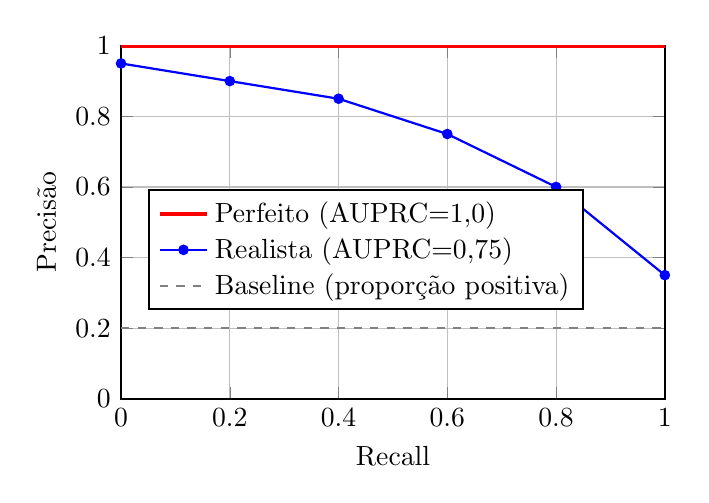
\begin{tikzpicture}
        \begin{axis}[
            width=0.7\textwidth,
            height=0.5\textwidth,
            xlabel={Recall},
            ylabel={Precisão},
            xmin=0, xmax=1,
            ymin=0, ymax=1,
            grid=major,
            % Ajustado: Legenda no canto inferior esquerdo, acima do baseline (y=0.25)
            legend style={at={(0.05,0.25)},anchor=south west}, 
            legend cell align={left},
            thick
        ]
        
        % Curva PR do Classificador Perfeito
        \addplot[color=red, ultra thick] coordinates {
            (0.0, 1.0)  
            (1.0, 1.0)  
        };
        \addlegendentry{Perfeito (AUPRC=1,0)}

        % Curva PR do Classificador Realista 
        \addplot[color=blue, thick, mark=*, mark size=1.5] coordinates {
            (0.0, 0.95)
            (0.2, 0.90)
            (0.4, 0.85)
            (0.6, 0.75)
            (0.8, 0.60)
            (1.0, 0.35)
        };
        \addlegendentry{Realista (AUPRC=0,75)}
        
        % Linha base (baseline)
        \addplot[dashed, color=gray] coordinates {
            (0,0.2) (1,0.2)
        };
        \addlegendentry{Baseline (proporção positiva)}
        
        \end{axis}
    \end{tikzpicture}
    
    \label{fig:pr_curve_comparison}
    \legend{Fonte: Elaborado pelo autor.}
\end{figure}

A curva azul ilustra o \textit{trade-off} de um modelo fictício. Conforme sua sensibilidade aumenta, ele começa a cometer erros de 
falso positivo, impactando negativamente a sua precisão. Na curva vermelha é ilustrada um modelo perfeito; nele esse \textit{trade-off}
não existe, o modelo sempre acerta, não importa o \textit{recall} \cite{geron2022hands}.

Em \citeonline{Mueller2016}, a AUCPR (\textit{area under curve precision recall} - ára sob a curva
precisão sensibilidade) é  definida como uma métrica que resume essas curvas. É possível comparar essa métrica com um \textit{baseline} que corresponde 
a um modelo que simplesmente adivinha; um acerto aleatório ou \textit{random guess}. No caso da curva PR, tal modelo teria um AUCPR igual a 
proporção da classe positiva. AUCPR é também chamada de AP (\textit{average precision} - precisão média).

Uma alternativa, segundo \citeonline{geron2022hands}, a curva PR é a curva ROC (\textit{receiver operating characteristic curve}) que exibe a sensibilidade em relação a taxa de falsos positivos. O seu 
comportamento é semelhante ao da curva PR, porém ela tende a ser otimista em conjunto de dados desbalanceados.
Assim, neste trabalho foi optado por usar apenas a curva PR. Porém, será discutido a AUC (\textit{area under the curve}) dos modelos. Essa métrica 
é equivalente a AUCPR, com a diferença que, para o \textit{baseline}, a AUC é sempre 0,5 \cite{Mueller2016}. Neste cenário, o \textit{recall} é igual à 
taxa de falsos positivos; ou seja, ao achar 60\% das classes positivas, o modelo classifica 60\% das classes negativas como positivas, por exemplo.
Um modelo perfeito, terá um AUC de 1,0 \cite{geron2022hands}.

\subsubsection{Curva de calibração}

\citeonline{mizilPredictingGoodProbs} apresentam uma definição visual de um modelo perfeitamente calibrado. 
No eixo x do diagrama estão intervalos, ou \textit{bins}, de probabilidade e no eixo y, a média da probabilidade prevista 
para um determinado intervalo. Agrupa-se as amostras em cada intervalo, de acordo com a probabilidade prevista e, então,
é calculado a média dessas probabilidades probabilidade e a frequência da classe positiva. Caso essas sejam iguais, então o modelo está 
perfeitamente calibrado.

Supondo que para um conjunto de pacientes, a média da probabilidade prevista é de 30\%. Se o modelo for perfeitamente
calibrado, então a frequência da classe positiva neste conjunto será de 30\%.

\begin{figure}[ht]
    \centering
    \caption{Diagrama de calibração mostrando curvas de modelos perfeitamente calibrado, superconfiante e subconfiante.}
    \label{fig:calibracao_exemplo}
    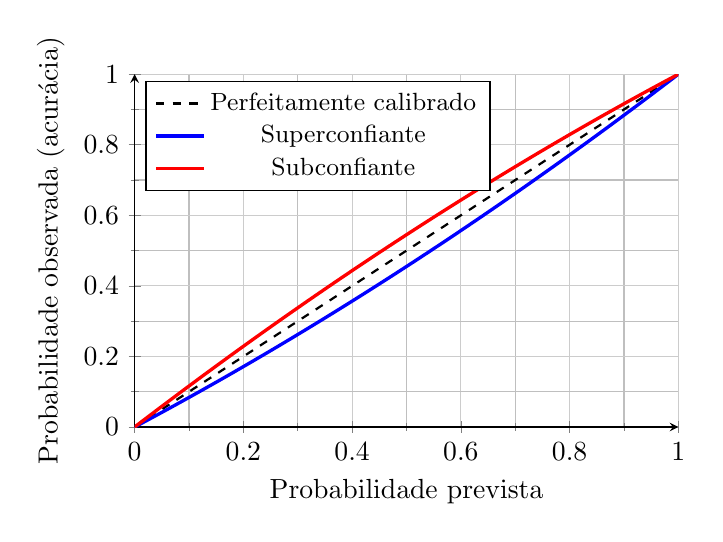
\begin{tikzpicture}
      \begin{axis}[
            width=0.7\textwidth,
            height=0.5\textwidth,
        xmin=0, xmax=1, ymin=0, ymax=1,
        xlabel={Probabilidade prevista},
        ylabel={Probabilidade observada (acurácia)},
        xtick={0,0.2,0.4,0.6,0.8,1},
        ytick={0,0.2,0.4,0.6,0.8,1},
        grid=both,
        major grid style={gray!40},
        minor tick num=1,
        legend style={at={(0.02,0.98)},anchor=north west,font=\small},
        axis lines=left
      ]

      % Linha perfeita (diagonal)
      \addplot [black, thick, dashed, domain=0:1, samples=201] {x};
      % Modelo superconfiante
      \addplot [blue, very thick, domain=0:1, samples=201, smooth] {x - 0.18*x*(1-x)};
      % Modelo subconfiante
      \addplot [red, very thick, domain=0:1, samples=201, smooth] {x + 0.18*x*(1-x)};

      \legend{Perfeitamente calibrado, Superconfiante, Subconfiante}
      \end{axis}
    \end{tikzpicture}
\end{figure}

Assim, um modelo perfeitamente calibrado tem uma curva correspondente a diagonal do diagrama. Modelos superconfiantes têm a sua curva 
abaixo da diagonal; a média das probabilidades previstas é maior que a frequência e modelos pouco confiantes têm a curva acima; a média 
das probabilidades previstas é menor que a frequência real.

\citeonline{mizilPredictingGoodProbs} afirmam que calibração é fundamental para a confiabilidade do modelo e não diretamente relacionado 
ao desempenho medido pelas demais métricas.